\markright{Implementation}
\section{Implementation}
\label{Implementation}
\definecolor{lightgray}{gray}{0.93}
  \vskip\baselineskip%
  \par\noindent\colorbox{lightgray}{%
    \begin{minipage}{0.98\textwidth}
		\textsc{Source Code}:\\
		The extended and working version of the code presented in this paper can be found on:\\
		\texttt{https://github.com/thoeni/rtos-project.git}
		\\There are two branches, the \texttt{main} and the \texttt{icecream} (which has been tested on \texttt{Android 4.0.1\_r1})
    \end{minipage}%
  }%
  \vskip\baselineskip%
As shortly described in the previous section, this small example relies on a native library we'll implement, and a summary of the flow from the Client Application (Activity named BbqueActivity) to the Server (Daemon named bbqued) can be seen in Fig. \ref{fig:projectoverview}.\\
\begin{figure}[!htb]
	\centering
	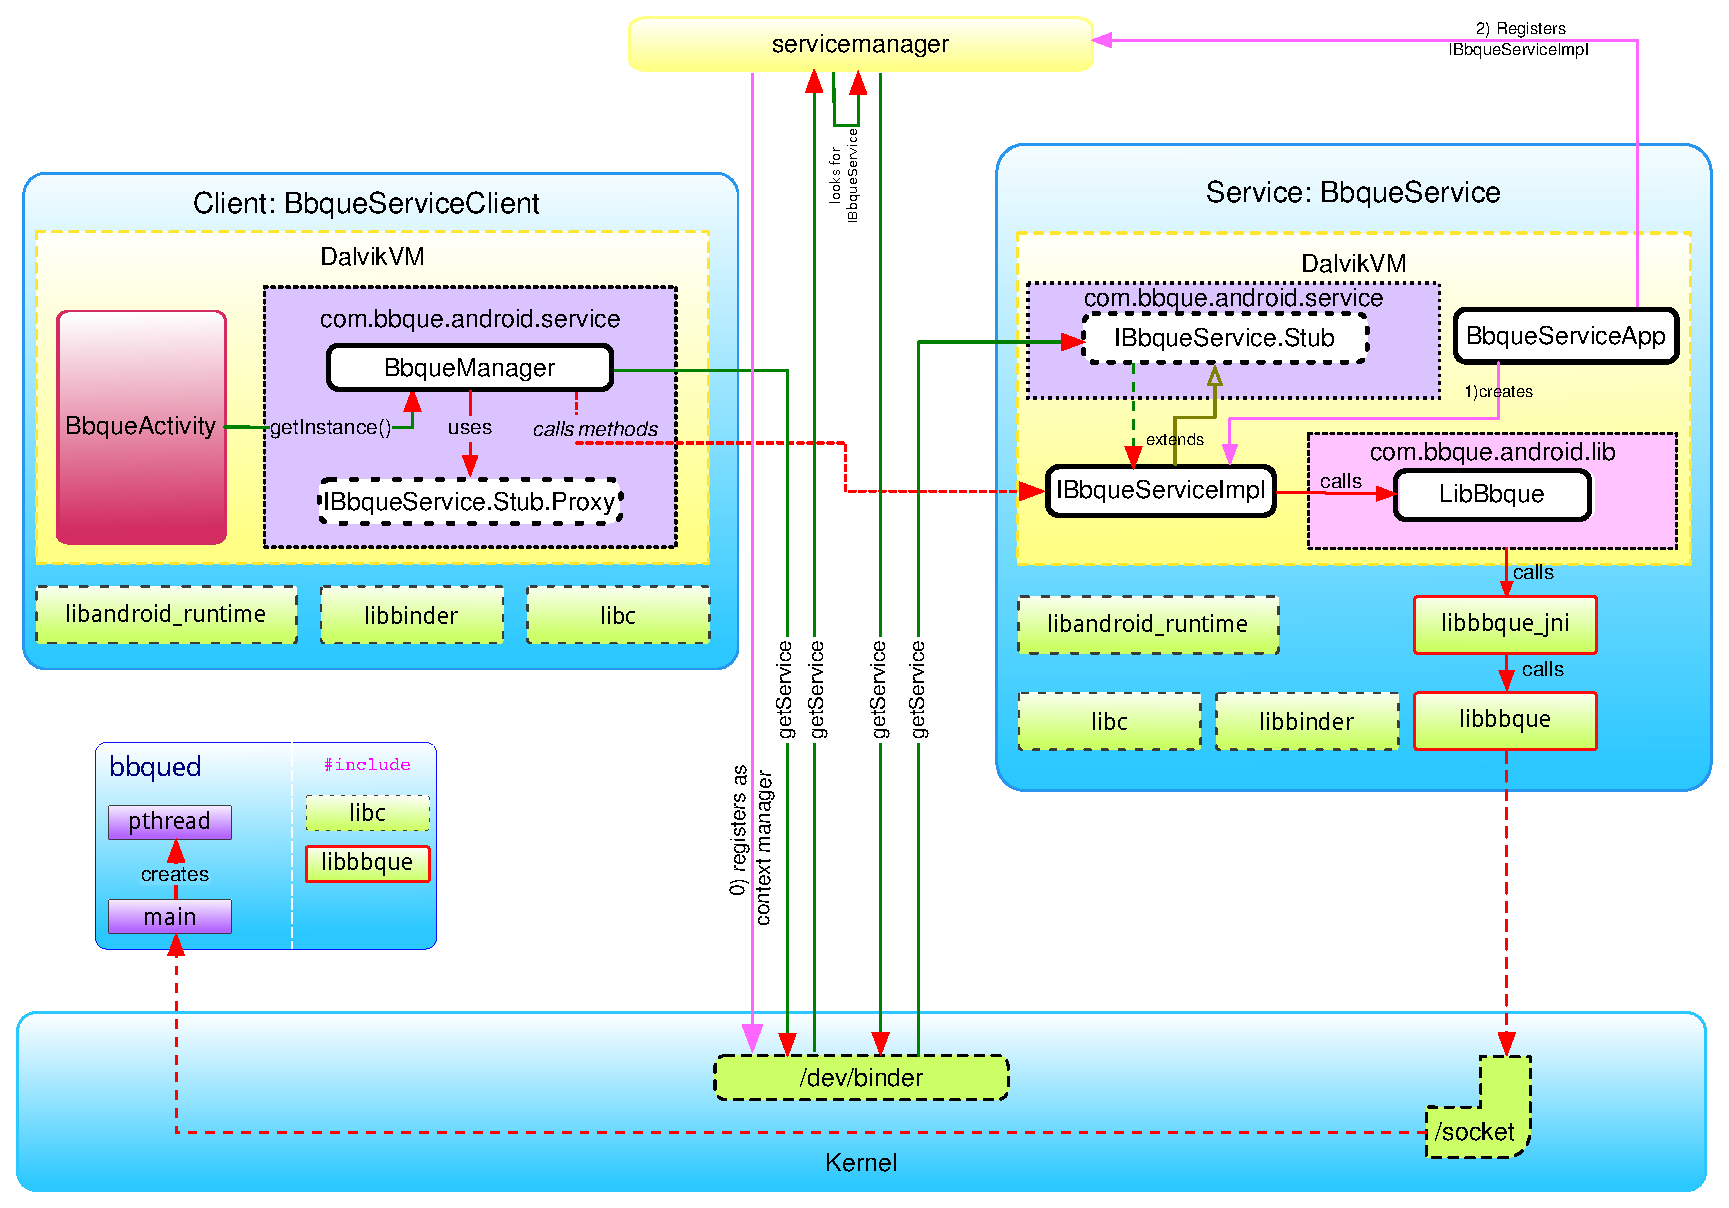
\includegraphics[scale=.432]{images/project_overview.pdf}
	\caption{Project flow overview}
	\label{fig:projectoverview}
\end{figure}
As a very high-level consideration, the modules on a \textbf{light blue} background run natively, while the modules over a \textbf{yellow} background run under Dalvik (therefore Java-coded). The \textbf{green} boxes are libraries, and the ones with a red stroke are included by our project. The \textbf{lilac} boxes are the two parts of our service, that communicate each other through binder. The \textbf{pink} box represents the Java module corresponding to our native library: the glue between them comes from JNI code. The flow indicated by the numbered \textbf{pink arrows} is executed during the startup phase.
\subsection{Native library}
Working directory for native library is \texttt{device/bosp/p2012-common/lib}.
The source tree for this directory is
\begin{verbatim}
lib/
|---Android.mk
|---libbbque/
    |---Android.mk
    |---libbbque.c
    |---libbbque.h
\end{verbatim}
The outermost \texttt{Android.mk} file contains just the instruction - for the building system - to search deeper for other \textit{makefiles}
\begin{verbatim}
	include $(call all-subdir-makefiles)
\end{verbatim}
The \texttt{libbbque} folder contains the \texttt{.h} header source with library's methods, \texttt{.c} source with library's methods implementation, along with another \texttt{Android.mk} file, which tells to the building system how to build this library module (eg. indicates the source file, the shared libraries to include, the name of the module, its optionality, and so on).\\
For the sake of clarity, we'll consider as example the
\begin{verbatim}
extern int get_core_availability() {
   [...]
   send_message_to_bbqued ("core", &core_number);
   return core_number;
}
\end{verbatim}
the inner method connects to the \texttt{bbqued} daemon through a socket, and sends his message, for instance the string \texttt{"core"}, saving the server's response into \texttt{int core\_number} variable.\\
To register the library module to the system, so that we can - natively - access to it, it's necessary to add to the \texttt{/p2012-common/bosp\_p2012.mk} the following line:
\begin{verbatim}
[...]
PRODUCT_PACKAGES += libbbque
\end{verbatim}
This line will append to the list of other \texttt{PRODUCT\_PACKAGES} string, our customised module, that will be added to the build-to-be version of Android.\\
The library can now be built, potentially as a stand-alone make operation, as follows:
\begin{verbatim}
$ . build/envsetup.sh
$ lunch full_bosp_p2012-eng
$ export USE_CCACHE=1
$ make -j8 libbbque
\end{verbatim}
\subsection{Native daemon}
Working directory for native daemon is \texttt{device/bosp/p2012-common/bin}.
\begin{verbatim}
bin/
|---Android.mk
|---bbqued/
|   |---Android.mk
|   |---bbqued.c
\end{verbatim}
The outermost \texttt{Android.mk} file is identical to the \texttt{lib/} case, while the inner one contains instructions to properly build the daemon module.\\
The \texttt{bbqued.c} file, which imports the \texttt{libbque.h} library, implements the server side of our test, which creates a \textit{socket} and waits for any incoming connection. When a connection is received, it launches a thread (implemented by using \texttt{pthread} library): each thread reads/writes an \texttt{int} variable which is local to the main process. As done for the library, the daemon module must be added to the \texttt{/p2012-common/bosp\_p2012.mk} file:
\begin{verbatim}
[...]
PRODUCT_PACKAGES += bbqued
\end{verbatim}
\definecolor{lightgray}{gray}{0.93}
  \par\noindent\colorbox{lightgray}{%
    \begin{minipage}{0.98\textwidth}
		\textsc{Adding the process to} \texttt{init.d}:\\
		After building the system, will be possible to run the daemon by accessing the system through \texttt{adb shell} command, and running the \texttt{bbqued} command (since it will be placed straight into \texttt{/bin} folder.\\
		If you want your process to be started at system startup, you can add it to the \texttt{init.d} file that you should have copied before as follows
		\vskip\baselineskip%
		\texttt{\$ cp system/core/rootdir/init.rc device/bosp/p2012-common/.}
		\vskip\baselineskip%	
		Then the building system must be notified to copy this customised file to the target \texttt{root} directory, as follows:
		\vskip\baselineskip%		
		\texttt{PRODUCT\_COPY\_FILES += \$(MY\_PATH)/init.rc:root/init.rc}
    \end{minipage}%
  }%
  \vskip\baselineskip%
To build this module, we have to make the system, as usual.
\subsection{Wrapping native library with JNI}
\label{JNIwrapping}
JNI is the glue to let C and Java talking to each other. This code will be put into directory \texttt{/p2012-common/framework/}, divided int two sub-directories as follows:
\begin{verbatim}
bbque_jni/
|---Android.mk
|---java/
|   |---Android.mk
|   |---com/
|   |   |---bbque/
|   |       |---android/
|   |           |---lib/
|   |               |---LibBbqueException.java
|   |               |---LibBbque.java
|   |---com.bbque.android.lib.xml
|---jni/
    |---Android.mk
    |---com_bbque_android_lib_LibBbque.c
    |---com_bbque_android_lib_LibBbque.h
\end{verbatim}
Create the \texttt{LibBbque.java} class, which contains just the declarations of the methods we want to expose to Java world (which must be declared as \texttt{public native}), as follows:
\begin{verbatim}
public native static int getNumCore() throws LibBbqueException;
\end{verbatim}
and the declaration of the jni library:
\begin{verbatim}
static {
   System.loadLibrary("bbque_jni");
}
\end{verbatim}
The \texttt{xml} file contains the declaration of permissions for the library, that will be generated as \texttt{jar} file during the next step:
\begin{verbatim}
<library name="com.bbque.android.lib"
    file="/system/framework/com.bbque.android.lib.jar"/>
\end{verbatim}
And finally the \texttt{Android.mk} file, under \texttt{java/} directory, h whicis quite elaborate, states all the instructions to properly compile the whole module that will be therefore included into the build process.\\
Then, the \texttt{make} command will process the module, and will generate a \texttt{classes.jar} file, which is needed by the next step, as input parameter to the \texttt{javah -jni} command, that generates the JNI header file.
\begin{verbatim}
$ javah -jni \
        -d device/bosp/p2012-common/framework/bbque_jni/jni/ \
        -classpath out/target/common/obj/JAVA_LIBRARIES/\ 
        com.bbque.android.lib_intermediates/classes-full-debug.jar \
        com.bbque.android.lib.LibBbque
\end{verbatim}
The first line suggests where the output header file will be placed, the second line gives as input the jar shared library generated during the previous step.\\
An example of an auto-generated signature, within the header file, is
\begin{verbatim}
JNIEXPORT jint JNICALL Java_com_bbque_android_lib_LiBbque_getNumCore
  (JNIEnv *, jclass);
\end{verbatim}
The next step consists into the implementation of the header file just generated, for example as follows:
\begin{verbatim}
JNIEXPORT jint JNICALL Java_com_bbque_android_lib_LiBbque_getNumCore
  (JNIEnv *env, jclass clazz) {
  jint result = get_core_availability();
  [...]
  }
\end{verbatim}
It's easy to realize that this is just a wrapping of the C native library.\\
After properly compiling the usual configuration files, \texttt{Android.mk} and the main \textit{makefile} \texttt{bosp\_p2012.mk} with the new modules to include, the system can be built again, and the native library is now accessible through \texttt{LibBbque} class:
\begin{verbatim}
LibBbque.getNumCore();
\end{verbatim}
We can say that the java call, so far, works within the upper right part of Fig. \ref{fig:projectoverview}, by calling Java methods on the \texttt{LibBbque} class (pink box).
\subsection{Binding the library with the Interface}
To let application-layer activities use the Java library previously created, an interface should be created, which will access to the library through \textit{Binder's} help.\\
To have an idea of the part of the flow in Fig. \ref{fig:projectoverview} we are working to, consider the greyed-out red-dashed-stroked area in Fig. \ref{fig:projectoverview_binder}.
\begin{figure}[!htb]
	\centering
	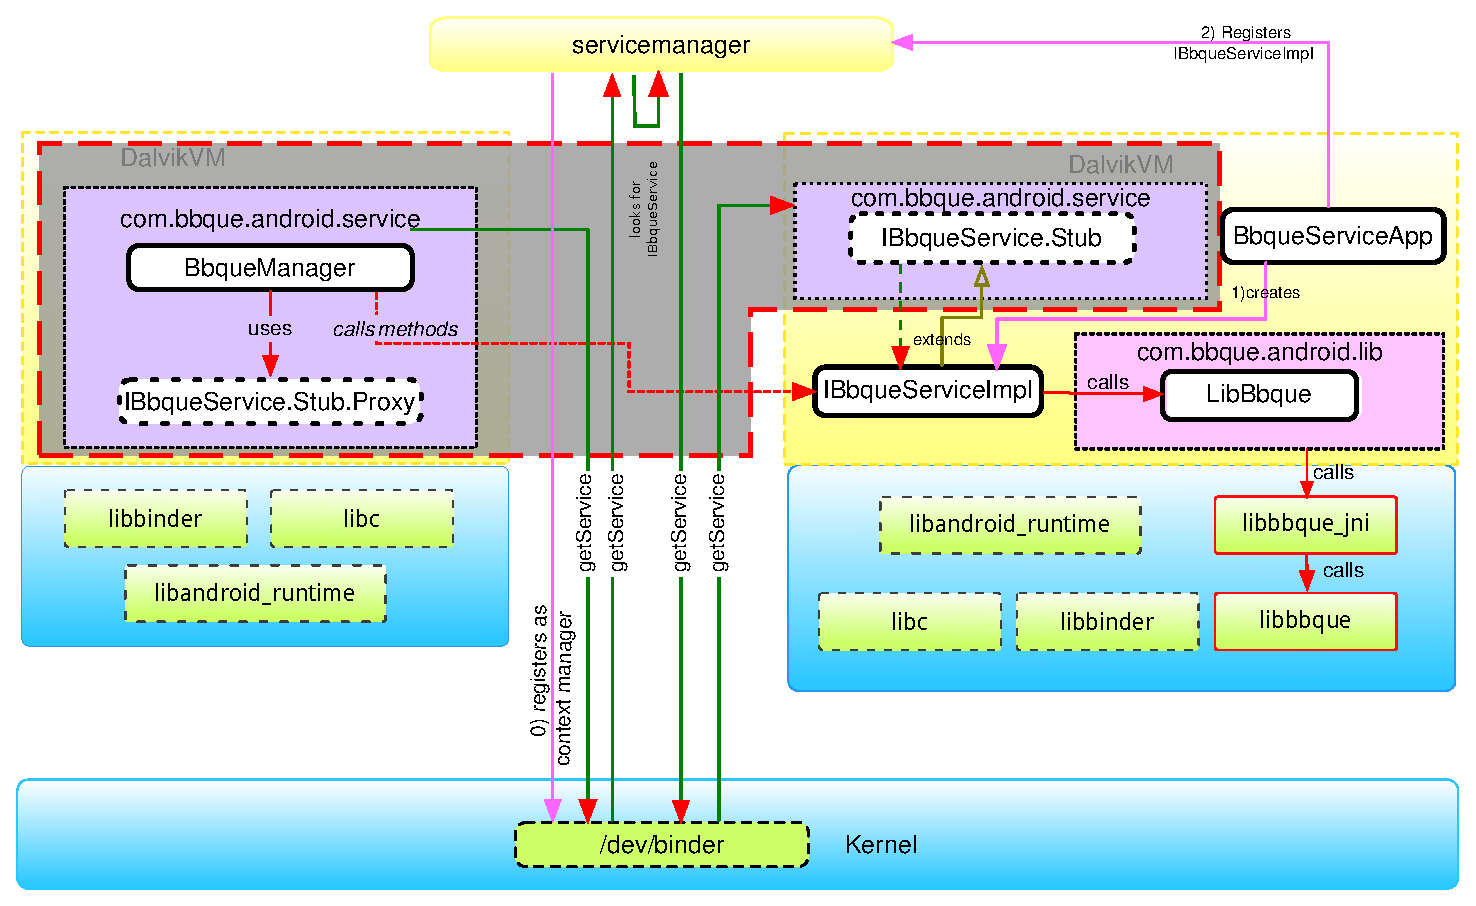
\includegraphics[scale=.505]{images/project_overview_binder.pdf}
	\caption{Interface-Library through binder}
	\label{fig:projectoverview_binder}
\end{figure}
\definecolor{lightgray}{gray}{0.93}
  \par\noindent\colorbox{lightgray}{%
    \begin{minipage}{0.98\textwidth}
		\textsc{RPC and Android Interface Definition Language}:\\
		Into Android, we do not use the Binder mechanism directly. Instead, we "define and interact with interfaces using Android's Interface Definition Language (IDL).
Interface definitions are usually stored in an \texttt{.aidl} file and are processed by the aidl tool to generate the proper stubs and marshalling/unmarshalling code required to transfer
objects and data back and forth using the Binder mechanism." \cite{embandroid}
    \end{minipage}%
  }%
  \vskip\baselineskip%
The working directory for this part is \texttt{bosp/p2012-common/framework/} where a new folder to include the interface and its manager has to be created (e.g. \texttt{bbqueservice}).
\begin{verbatim}
bbqueservice/
|---Android.mk
|---com/
|   |---bbque/
|       |---android/
|           |---service/
|               |---BbqueManager.java
|               |---IBbqueService.aidl
|---com.bbque.android.service.xml
\end{verbatim}
As seen for the previous module, \texttt{xml} file contains permissions declaration, and \texttt{Android.mk} file contains instructions for the building system to properly compile the module. Going deeper into folder's tree, there are two files:
\begin{itemize}
	\item \texttt{IBbqueService.aidl}\\
		As stated in the grey-coloured note above, this interface contains the methods' definitions. An example for our testing case is
		\begin{verbatim}
			interface IBbqueService {
			   int getNumCore();
			   [...]
			}
		\end{verbatim}
	\item \texttt{BbqueManager.java}\\
	This class is a proxy to our bounded service, and will be instantiated bu any Application that will need to access to the Interface. It mainly returns the interface to the caller, as follows:
	\begin{verbatim}
		[...]
		import android.os.IBinder;
		import android.os.ServiceManager;
		[...]
		private final IBbqueService service;
		this.service = IBbqueService.Stub.asInterface(
		               ServiceManager.getService(REMOTE_SERVICE_NAME));
		[...]
	\end{verbatim}
\end{itemize}
\subsection{ServiceManager registering and Interface implementation}
Regarding the previous lines, to let the \texttt{BbqueManager} get the desired service, by calling the \texttt{ServiceManager.getService(...)} method, we must register our service into the Service Manager, otherwise it can't find - and therefore return - it to the caller. This operation is performed by a class called \texttt{BbqueServiceApp}. In Fig. \ref{fig:projectoverview_serviceapp} a portion of Fig. \ref{fig:projectoverview} focusing on this part can be seen.
\begin{figure}[!htb]
	\centering
	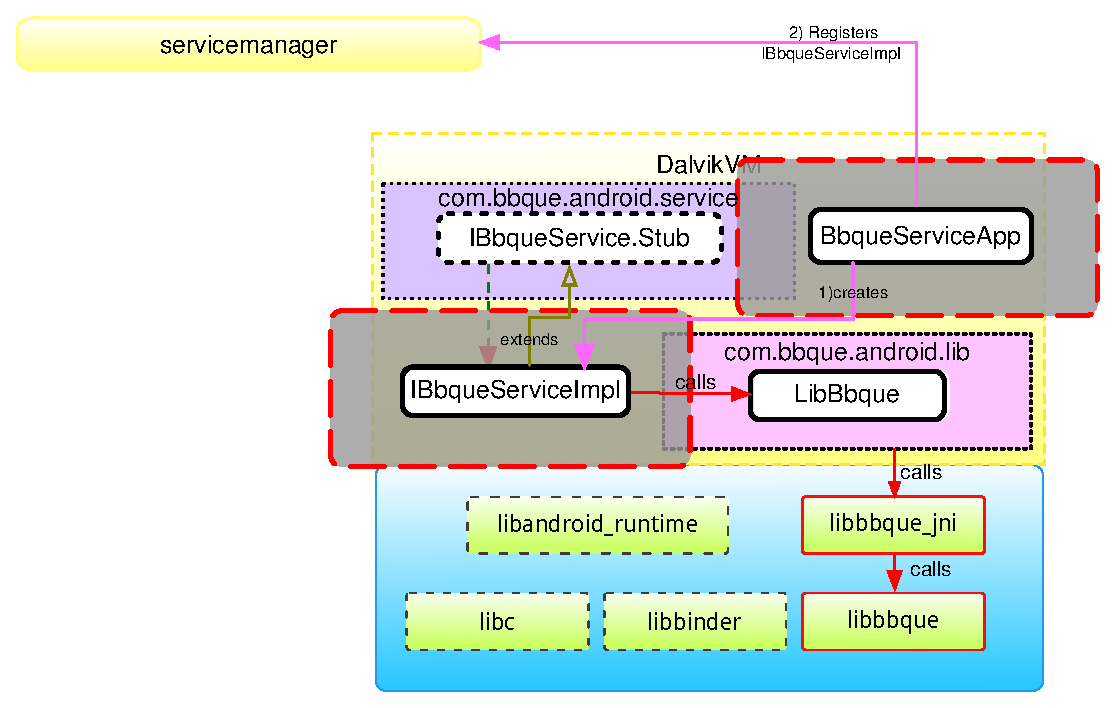
\includegraphics[scale=.505]{images/project_overview_IServiceImpl.pdf}
	\caption{Interaction ServiceApp - ServiceManager}
	\label{fig:projectoverview_serviceapp}
\end{figure}
The working directory is \texttt{bosp/p2012-common/app/}. Follows a tree summary within this folder.
\begin{verbatim}
app/
|---Android.mk
|---BbqueService
    |---AndroidManifest.xml
    |---Android.mk
    |---src
        |---com
            |---bbque
                |---android
                    |---bbqueservice
                        |---BbqueServiceApp.java
                        |---IBbqueServiceImpl.java
\end{verbatim}
\texttt{AndroidManifest.xml} file contains the declarations of the server application.\\
The inner \texttt{BbqueServiceApp.java} class, is declared as
\begin{verbatim}
public class BbqueServiceApp extends Application
\end{verbatim}
and \textit{overloads} the \texttt{onLoad} inherited method, with the \texttt{IBbqueServiceImpl} object creation, and its registration to the ServiceManager (pink arrows in Fig. \ref{fig:projectoverview_serviceapp}).
\begin{verbatim}
this.serviceImpl = new IBbqueServiceImpl(this);
ServiceManager.addService(REMOTE_SERVICE_NAME, this.serviceImpl);
\end{verbatim}
The \texttt{IBbqueServiceImpl.java} class, is declared as
\begin{verbatim}
class IBbqueServiceImpl extends IBbqueService.Stub
\end{verbatim}
and defines a constructor which takes as input a \texttt{Context} variable, and a simple \texttt{return} statement for each desired method we want to expose.\\
Finally, the last step before another building process, is to add this package to the main \textit{makefile} that, in our case, is \texttt{p2012-common/bosp\_p2012.mk}:
\begin{verbatim}
PRODUCT_PACKAGES += BbqueService
\end{verbatim}
As already seen before, the \texttt{+=} symbol, appends this last definition to all the others, to contribute to the creation of the main \textit{makefile}.\\
Android's log, during the startup, shows the following lines:
\begin{verbatim}
I/ActivityManager(  147): Start proc com.bbque.android.bbqueservice
               for added application com.bbque.android.bbqueservice:
               pid=242 uid=1000 gids={1015, 3002, 3001, 3003, 1028}
               
D/BbqueServiceApp(  242): Registered 
               [com.bbque.android.bbqueservice.IBbqueServiceImpl] as
               [com.bbque.android.service.IBbqueService]
\end{verbatim}
\subsection{Application layer}
At this phase, everything is ready to be used by any Android Application/Activity. In Fig. \ref{fig:screenshot} a very simple application made to test the calls' flow, and in Fig. \ref{fig:shell} the \texttt{\$ adb logcat} output for a \texttt{get\_core\_availability()} call.
\begin{figure}[!htb]
	\centering
	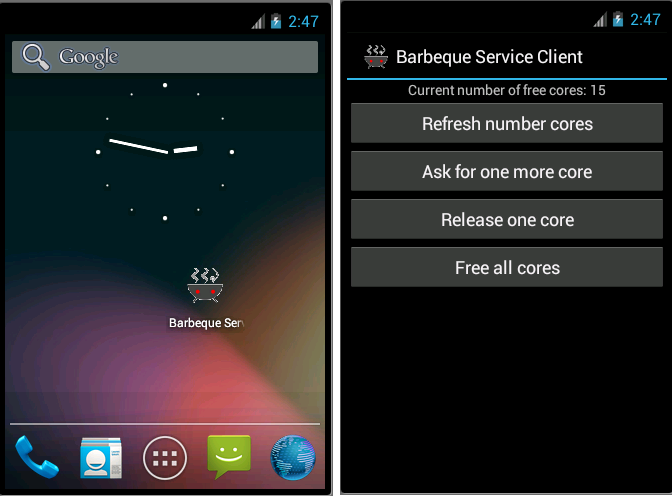
\includegraphics[scale=.505]{images/screenshot_duo.png}
	\caption{Home screen (left), Sample app (right)}
	\label{fig:screenshot}
\end{figure}
\begin{figure}[!htb]
	\centering
	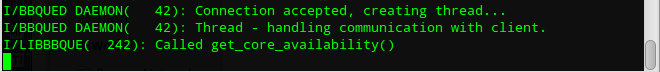
\includegraphics[scale=.505]{images/shell.png}
	\caption{Shell - Straight call}
	\label{fig:shell}
\end{figure}
\subsection{The other way around - callback}
If we wanted to see an example of how a similar call can go the opposite direction, we should implement a C-to-Java callback paradigm.\\
As long as I've seen, to achieve this result, the \textit{callback} approach requires - as the word itself clearly suggests - a first call from Java to C. Doing so, Java will pass to the native code (as previously seen in \ref{JNIwrapping}) some parameters as \texttt{JNIEnv} and \texttt{jclass}. Through these pointers, and some convenient specific functions, the native code is able to \textit{callback} a method coded within the Java class that made the first call: as long as the native process can hold the proper references to JNIEnv (or, actually, the global JavaVM, from which it can get back the environment) it will be able to make asynchronous calls to the Java methods belonging to the caller.\\
We'll briefly see the code used to achieve this which, at the moment of this writing, is contained into the Git \texttt{jb-callback} branch.
\begin{enumerate}
	\item The Java library \texttt{LibBbque} class (seen in \ref{JNIwrapping}) contains the following methods:
	\begin{verbatim}
		public native static int sendMessageToApp();
		
		public static void appCallback() {
		   System.out.println("JNI works.");
		}
	\end{verbatim}
	The former is needed to call the native library, and pass it the JNI parameters, while the latter is the class' method that C library will execute.
	\item As done before, after a \texttt{make} command, the JNI header file will be generated through a \texttt{javah -jni [...]} command. The result is
	\begin{verbatim}
		/*
		 * Class:     com_bbque_android_lib_LibBbque
		 * Method:    sendMessageToApp
		 * Signature: ()I
		 */
		 
		JNIEXPORT jint JNICALL
		          Java_com_bbque_android_lib_LibBbque_sendMessageToApp
		          (JNIEnv *, jclass);
	\end{verbatim}
	Its implementation will include the C native library, and call the native function:
	\begin{verbatim}
		#include <libbbque.h>
		#include "com_bbque_android_lib_LibBbque.h"
		[...]
		JNIEXPORT jint JNICALL
		          Java_com_bbque_android_lib_LibBbque_sendMessageToApp
		          (JNIEnv *env, jclass clazz) {
		             jint result = send_message_to_app(env, clazz);
		          [...]
		          }
	\end{verbatim}
	\item The callback implementation is mainly coded into this last native piece of code: the native library, \texttt{libbbque.c}
	\begin{verbatim}
		extern int send_message_to_app(JNIEnv *env, jclass clazz) {
		  __android_log_write(ANDROID_LOG_INFO, LOG_TAG,
		                      "Called send_message_to_app()");
		  jmethodID mid = (*env)->GetStaticMethodID (env, 
		                                             clazz,
		                                             "appCallback",
		                                             "()V");
		  (*env)->CallStaticVoidMethod(env, clazz, mid);
		  __android_log_write(ANDROID_LOG_DEBUG, LOG_TAG,
		                      "...method called back!");	
		  return 0;
		}
	\end{verbatim}
	This code allows a synchronous one-shot callback: the \texttt{GetStaticMethodId} looks for the \texttt{appCallback} method, with \texttt{()V} signature into the caller class: this means it will search for a \texttt{static void appCallback()} method. Its output fill be saved to \texttt{jmethodID} variable. This variable will be given as input parameter to the \texttt{CallStaticVoidMethod} method, to execute the callback.
	\item To test this implementation, we can let the Activity call the Java method which \textit{"opens"} the communication with C native library, by sending down the stack its JNIEnv and jclass data, as follows:
	\begin{verbatim}
		 public void run() {
		   [...]
		   this.bbqueManager.sendMessageToApp();
		 }
	\end{verbatim}
	The result of Activity launching, into the \texttt{catlog} screen is shown in Fig. \ref{fig:shell2}
\end{enumerate}
\begin{figure}[!htb]
	\centering
	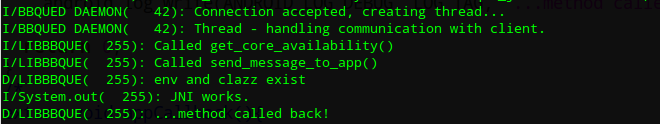
\includegraphics[scale=.505]{images/shell2.png}
	\caption{Shell - callback}
	\label{fig:shell2}
\end{figure}
The code of the native library could also save some global references (to be used asynchronously by any running process) as follows:
\begin{verbatim}
	//Saving GlobalJVM
	(*env)->GetJavaVM(env, &global_jvm);
	//Saving GlobalClass
	libbbque_global_class = (*env)->NewGlobalRef(env, clazz);
\end{verbatim}
These references should be passed to any daemon or running process, for future use, before the library loses them. This passage hasn't been implemented yet.